\documentclass[tikz,border=5pt]{standalone}

\usepackage{pgfplots}
\pgfplotsset{compat=1.18}

\begin{document}

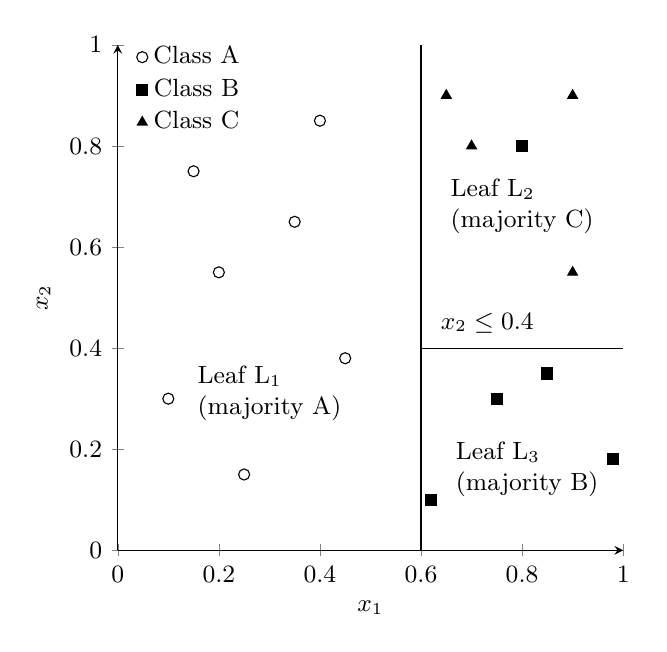
\begin{tikzpicture}
    \begin{axis}[
        width=8cm,height=8cm,
        xmin=0,xmax=1,ymin=0,ymax=1,
        xlabel={$x_1$},ylabel={$x_2$},
        axis x line=bottom, axis y line=left,
        xtick={0,0.2,0.4,0.6,0.8,1.0},
        ytick={0,0.2,0.4,0.6,0.8,1.0},
        tick label style={font=\small},
        label style={font=\small},
        legend style={draw=none,fill=none,at={(0.02,1.02)},anchor=north west,font=\small}
    ]
        % Class A (circles)
        \addplot[only marks,mark=o,mark size=2pt] coordinates {
            (0.15,0.75) (0.20,0.55) (0.35,0.65) (0.40,0.85) (0.10,0.30)
            (0.25,0.15) (0.45,0.38)
        };
        % Class B (squares)
        \addplot[only marks,mark=square*,mark size=2pt] coordinates {
            (0.80,0.80) (0.75,0.30) (0.98,0.18)
            (0.62,0.10) (0.85,0.35)
        };

        % Class C (triangles)
        \addplot[only marks,mark=triangle*,mark size=2pt] coordinates {
            (0.70,0.80) (0.90,0.55) (0.65, 0.90) (0.90,0.90)
        };

        \legend{Class A, Class B, Class C}
    
        % Split 1: x1 <= 0.6
        \addplot[domain=0:1, samples=2] ({0.6},{x});
        \node[font=\small,anchor=south] at (axis cs:0.55,1.1) {$x_1 \le 0.6$};
    
        % Split 2 (right child): x2 <= 0.4
        \addplot[domain=0.6:1, samples=2] ({x},{0.4});
        \node[font=\small,anchor=west] at (axis cs:0.62,0.45) {$x_2 \le 0.4$};
    
        % Region labels (leaves)
        \node[font=\small,align=left] at (axis cs:0.30,0.31) {Leaf L$_1$\\(majority A)};
        \node[font=\small,align=left] at (axis cs:0.80,0.68) {Leaf L$_2$\\(majority C)};
        \node[font=\small,align=left] at (axis cs:0.81,0.16) {Leaf L$_3$\\(majority B)};
    \end{axis}
\end{tikzpicture}

\end{document}
